\section{Study Area}
\label{sec:study_area}

The \emph{Stagnone di Marsala} is sheltered from the Sicilian channel by Isola
Grande, an elongated barrier island parallel to the mainland coast
(Figure~\ref{fig:study_area}). The basin extends about 11~km north--south and
2.5~km east--west over roughly 2200~ha \citep{DeMarchis2012}, and a
\emph{P.\ oceanica} barrier reef divides it into a northern sub-basin of about
1~m mean depth with extensive intertidal flats and a southern sub-basin of
about 2~m, reaching 3~m near the main inlet \citep{LaLoggia2004}. Three
islands lie in the interior, Mothia, the site of a Phoenician settlement, in
the south-central basin and Santa Maria and Scuola in the central reaches
\citep{CiraoloDeMarchis2009}, and salt pans occupy both margins, on Isola
Grande and along the mainland shore facing Mothia \citep{Basso2008}.

The lagoon exchanges with the open sea through two inlets. The northern inlet,
about 400~m wide and 0.30--0.40~m deep, is restricted by its sill, which a
dredged channel 20~m wide and 1~m deep partly bypasses, and the southern inlet,
about 2900~m wide and 1.0--1.5~m deep, carries most of the exchange and mixing
with the open sea \citep{CiraoloDeMarchis2009}. The tide is microtidal, with
amplitudes of about 0.30~m dominated by semi-diurnal harmonics
\citep{LaLoggia2004}. Wind drives the east--west circulation within the basin
and tidal exchange its north--south component \citep{CiraoloDeMarchis2009,
DeMarchis2012}. With no riverine input, weak exchange and high summer
evaporation produce a salinity gradient, annual values spanning 33--46
\citep{Basso2008} and summer values approaching 48 in the confined northern
sub-basin against near-marine conditions at the southern inlet
\citep{Mancuso2023}.

Seagrass covers most of the lagoon floor, \emph{P.\ oceanica} occupying the
central and southern basin in continuous meadows and atolls 10--20~m in
diameter that grade into reefs aligned north--south, and \emph{C.\ nodosa}
prevailing in the shallower north, with \emph{Caulerpa prolifera} replacing
\emph{P.\ oceanica} locally where hydrodynamic and sediment conditions
deteriorate \citep{LaLoggia2004, CiraoloDeMarchis2009}. \emph{P.\ oceanica}
reaches 1000--1200 plants~\si{\per\metre\squared} in Mediterranean meadows of
this type \citep{Ciraolo2009a}. The submerged vegetation was first mapped from
airborne hyperspectral imagery by \citet{CiraoloMaltese2006}, and the canopy
in this study rests on a classification of PlanetScope imagery of 2023
(Section~\ref{sec:methods_roughness}). The lagoon is a \emph{Riserva Naturale
Orientata} and a Natura 2000 site, and satellite monitoring has nevertheless
documented a reduction of about 75\% in the extent of the atoll and cordon
formations between 2003 and 2024 \citep{Maltese2025}.

The observations were collected in July 2025 (Figure~\ref{fig:study_area}).
Water level was recorded at the North Mouth (NM), at the South Mouth (SM) and
at AltaVilaEst (AE) in the northern basin, the last also carrying wind,
pressure and water temperature sensors, and a second meteorological station,
Mulino, stands near the salt pans of the central-northern margin. The tide
gauge on Marettimo island (JRC TAD 658), about 35~km to the west, gives an
offshore reference free of lagoon dynamics, and GPS-tracked surface drifters
were released in the lagoon interior within the simulation window
(Section~\ref{sec:methods_validation}).

%% Produced by scripts/plot_study_area_paper1.py
\begin{figure}[!htbp]
  \centering
  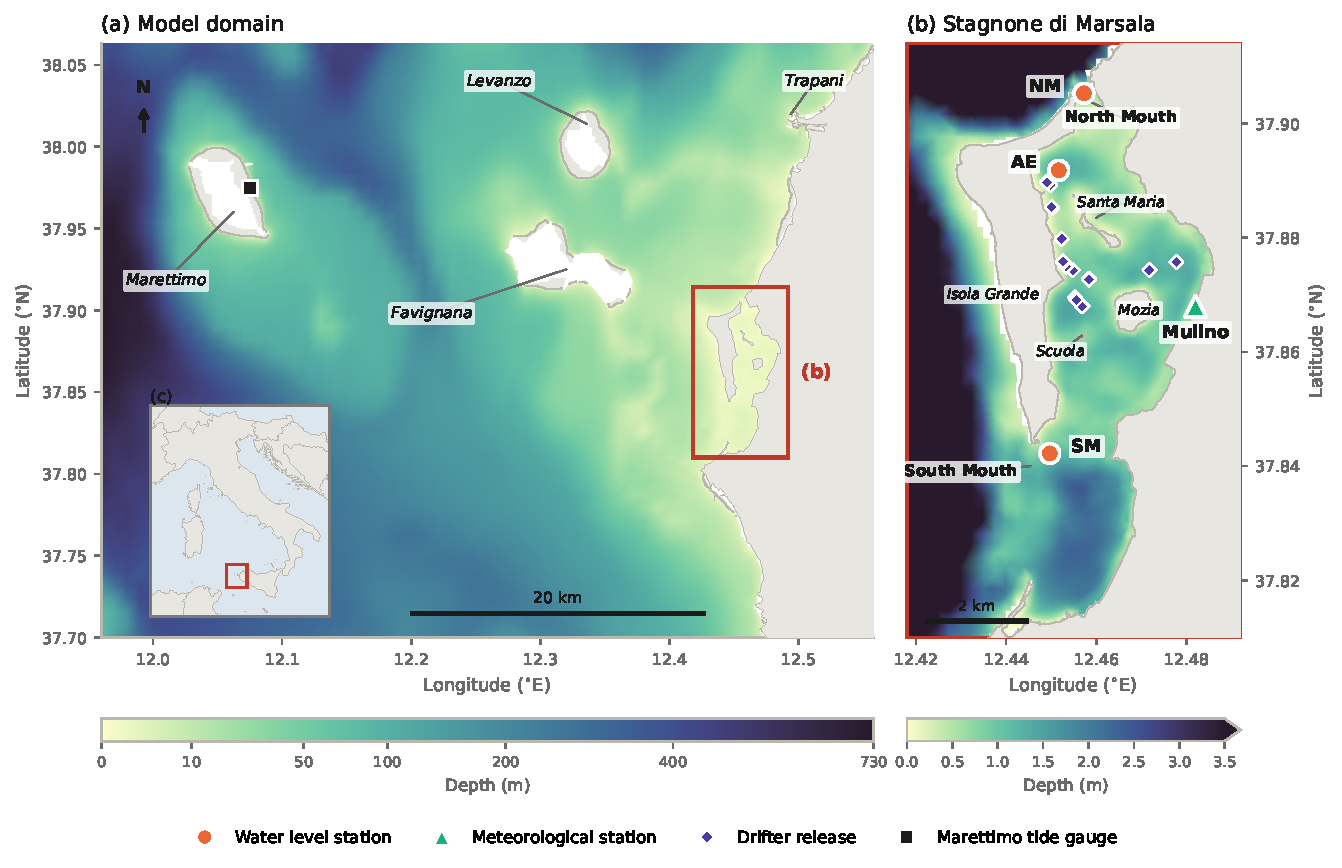
\includegraphics[width=\textwidth]{study_area_stagnone}
  \caption{The study area. (a) The modelled domain, covering western Sicily,
  the Egadi archipelago and the adjacent shelf, with the Marettimo tide gauge
  used for offshore validation. The red box gives the extent of panel (b).
  (b) The Stagnone di Marsala, with the water level stations North Mouth (NM),
  AltaVilaEst (AE) and South Mouth (SM), the Mulino meteorological station,
  and the 35 GPS drifter release positions of the twelve July 2025
  deployments. (c) The domain within Italy. Colour gives depth below the
  reference level on the model mesh, on separate scales for (a) and (b).}
  \label{fig:study_area}
\end{figure}
